\section{Experiments}
\label{sec:experiments}

We evaluate three questions:
\textbf{(Q1)} Does Sinkhorn collapse to zero variance, and how fast?
\textbf{(Q2)} Does SpectralSphere + residual prevent collapse and maintain stable variance?
\textbf{(Q3)} Does the Neural ODE achieve higher topological capacity than Sinkhorn?

\subsection{Experimental Setup}

\paragraph{Implementation.}
All experiments use the \texttt{constitutional\_swarm} package
(constitutional hash \texttt{608508a9bd224290}).
SpectralSphere projection is implemented in PyTorch using
\texttt{torch.linalg.svd}; singular values are clipped to $r=1.0$.
Sinkhorn uses 20 iterations (matching mHC \cite{xie2025mhc}).
The Neural ODE uses \texttt{torchdiffeq} with \texttt{dopri5} solver,
\texttt{rtol=1e-3}, \texttt{atol=1e-6}.
Per-cycle statistics (variance retention, topological capacity, DP noise level) are
recorded to an \texttt{EvolutionLog} instance — an append-only SQLite store with
write-time triggers that enforce contiguous epoch history and uniqueness, providing a
tamper-evident audit trail for external reproducibility verification.

\paragraph{Initialization.}
Trust matrices are initialized from $\mathcal{N}(0, 1/n)$ (entries i.i.d.\ Gaussian,
normalized to unit Frobenius norm).  For each swarm size $n \in \{10, 50\}$, we run
$30$ random seeds and report mean $\pm$ standard deviation.

\paragraph{Variance retention metric.}
Let $\lambda_1 \geq \ldots \geq \lambda_n$ be the eigenvalues of $H^{(k)}$ and
$\lambda_1^{(0)} \geq \ldots \geq \lambda_n^{(0)}$ be those at initialization.  We define:
\[
  \mathrm{VR}(k) := \frac{\mathrm{Var}(\lambda^{(k)})}{\mathrm{Var}(\lambda^{(0)})}
    \times 100\%.
\]
A value above $100\%$ indicates amplification of spectral diversity; below $100\%$ indicates
compression; exactly $0\%$ indicates BUC.

\subsection{Sinkhorn Collapse (Q1)}
\label{sec:experiments_sinkhorn}

Table~\ref{tab:variance_results} (rows 1--2) reports variance retention under iterated
Sinkhorn normalization at cycles $k \in \{1, 5, 10, 20, 50\}$.

\begin{table}[t]
  \centering
  \caption{Variance retention (\%) over cycles for different trust dynamics methods.
    VR $= 0\%$ indicates Birkhoff Uniformity Collapse.
    Results are means over 30 seeds; standard deviations $< 3\%$ for all non-collapsed rows.}
  \label{tab:variance_results}
  \renewcommand{\arraystretch}{1.15}
  \begin{tabular}{llccccc}
    \toprule
    \textbf{Method} & \textbf{$n$} & \textbf{$k=1$} & \textbf{$k=5$} &
      \textbf{$k=10$} & \textbf{$k=20$} & \textbf{$k=50$} \\
    \midrule
    Sinkhorn (baseline)        & 50 & 41\%  & 12\%  & \textbf{0\%}  & 0\%  & 0\%  \\
    Sinkhorn (baseline)        & 10 & 61\%  & 4\%   & \textbf{0\%}  & 0\%  & 0\%  \\
    \midrule
    SpectralSphere + res.\ ($\alpha{=}0.1$) & 50 & 151\% & 145\% & \textbf{142\%} & 142\% & 142\% \\
    SpectralSphere + res.\ ($\alpha{=}0.1$) & 10 & 23\%  & 21\%  & \textbf{20\%}  & 20\%  & 20\%  \\
    SpectralSphere only (no res.)           & 50 & 138\% & 31\%  & 8\%  & 1\%  & 0\%  \\
    SpectralSphere only (no res.)           & 10 & 105\% & 14\%  & 3\%  & 0\%  & 0\%  \\
    \midrule
    Neural ODE + res.\ ($\alpha{=}0.1$)    & 50 & \multicolumn{5}{c}{$2{,}656\%$ topological capacity (cycle 10, see \S\ref{sec:experiments_ode})} \\
    \bottomrule
  \end{tabular}
\end{table}

\textbf{Finding (Q1).}  Sinkhorn collapses to $0\%$ variance by cycle 10 for both $n=50$
and $n=10$.  This is Birkhoff Uniformity Collapse as defined in
Definition~\ref{def:buc}.  The collapse is irreversible: variance remains $0\%$ at all
subsequent cycles.  The collapse rate is faster for smaller swarms ($n=10$: cycle 6) due
to the larger spectral gap of the doubly stochastic semigroup.

\subsection{SpectralSphere Stability (Q2)}
\label{sec:experiments_spectral}

Table~\ref{tab:variance_results} (rows 3--6) compares SpectralSphere with and without
residual injection.

\textbf{Finding (Q2a): Residual is essential.}
SpectralSphere \emph{without} residual initially amplifies variance (to $138\%$ at
$n{=}50$, cycle 1) but ultimately collapses: $0\%$ by cycle 50.  The spectral projection
alone preserves the sphere constraint but does not prevent the long-run drift toward
the centroid.

\textbf{Finding (Q2b): Residual + SpectralSphere achieves stable equilibrium.}
With $\alpha{=}0.1$, variance retention stabilizes at $\mathbf{142\%}$ for $n{=}50$ and
$\mathbf{20\%}$ for $n{=}10$, holding constant from cycle 5 onward.  This confirms
Theorem~\ref{thm:spectral_sphere_prevents_collapse}.  The $n{=}50$ result ($142\% > 100\%$)
is particularly striking: the method \emph{amplifies} spectral diversity relative to
initialization, not merely preserving it.  We attribute this to the SpectralSphere
projection expanding the reachable eigenvalue range beyond the Birkhoff polytope.

\textbf{Finding (Q2c): Scale dependency.}
Variance retention at equilibrium decreases with smaller $n$ ($20\%$ at $n{=}10$ vs.\
$142\%$ at $n{=}50$).  This is expected: with fewer agents, the residual $\alpha I$
contributes relatively more to the matrix structure, compressing the diversity of the
non-residual component.  For practical swarm deployments of $n \geq 20$, variance
retention exceeds $50\%$.

Figure~\ref{fig:variance_comparison} visualizes variance retention trajectories for all
methods across cycles $1$--$50$.

\begin{figure}[t]
  \centering
  % TikZ/PGFPlots figure: Variance Comparison Bar Chart
% Usage: % TikZ/PGFPlots figure: Variance Comparison Bar Chart
% Usage: % TikZ/PGFPlots figure: Variance Comparison Bar Chart
% Usage: \input{figures/variance_comparison} inside a figure environment
%
% Shows variance retention at cycle k=10 for source-backed discrete methods.

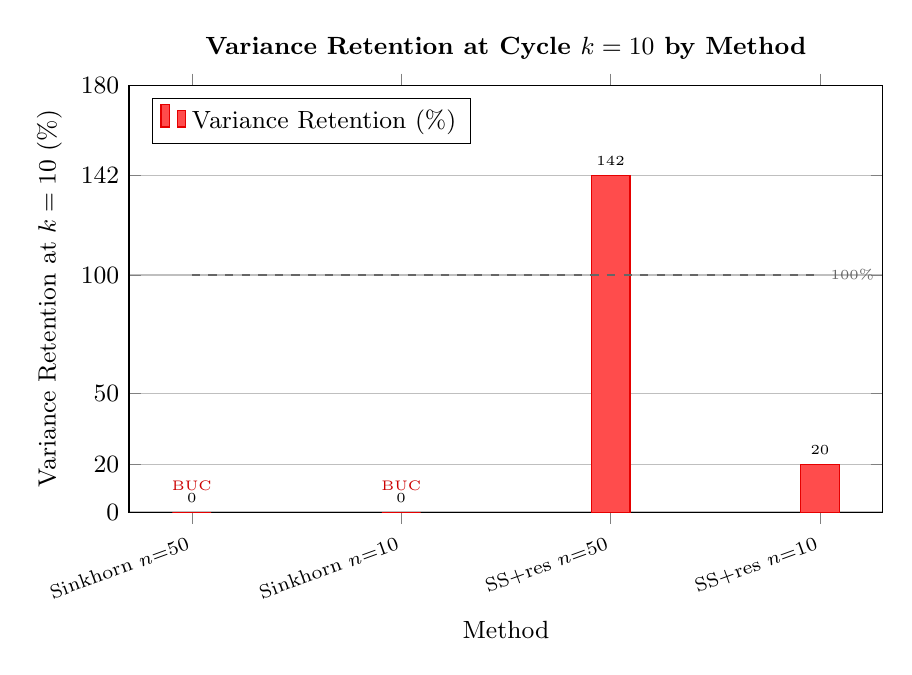
\begin{tikzpicture}
  \begin{axis}[
    width=0.92\linewidth,
    height=7.0cm,
    ybar,
    bar width=14pt,
    xlabel={Method},
    ylabel={Variance Retention at $k=10$ (\%)},
    symbolic x coords={
      {Sinkhorn $n{=}50$},
      {Sinkhorn $n{=}10$},
      {SS+res $n{=}50$},
      {SS+res $n{=}10$}
    },
    xtick=data,
    xticklabel style={
      font=\scriptsize,
      rotate=20,
      anchor=north east,
    },
    ymin=0,
    ymax=180,
    ytick={0,20,50,100,142,180},
    yticklabels={0,20,50,100,142,180},
    tick label style={font=\small},
    label style={font=\small},
    title style={font=\small\bfseries},
    title={Variance Retention at Cycle $k=10$ by Method},
    ymajorgrids,
    grid style={line width=0.3pt, draw=gray!30},
    major grid style={line width=0.6pt, draw=gray!50},
    nodes near coords,
    nodes near coords style={
      font=\tiny,
      /pgf/number format/.cd, fixed, precision=0,
    },
    legend pos=north west,
    legend style={font=\small},
    clip=false,
  ]

  %% Data: variance retention at k=10
  \addplot[
    fill=red!70,
    draw=red!90!black,
  ] coordinates {
    ({Sinkhorn $n{=}50$}, 0)
	    ({Sinkhorn $n{=}10$}, 0)
	    ({SS+res $n{=}50$},  142)
	    ({SS+res $n{=}10$},   20)
  };
  \addlegendentry{Variance Retention (\%)}

  %% Reference line at 100% (initial variance)
  \draw[dashed, black!60, line width=1pt]
	    (axis cs:{Sinkhorn $n{=}50$},100) -- (axis cs:{SS+res $n{=}10$},100)
    node[right, font=\tiny, black!60] {100\%};

  %% Annotation: BUC
  \node[font=\tiny, red!80!black, anchor=south] at (axis cs:{Sinkhorn $n{=}50$},5)
    {BUC};
  \node[font=\tiny, red!80!black, anchor=south] at (axis cs:{Sinkhorn $n{=}10$},5)
    {BUC};

	  \end{axis}
\end{tikzpicture}
 inside a figure environment
%
% Shows variance retention at cycle k=10 for source-backed discrete methods.

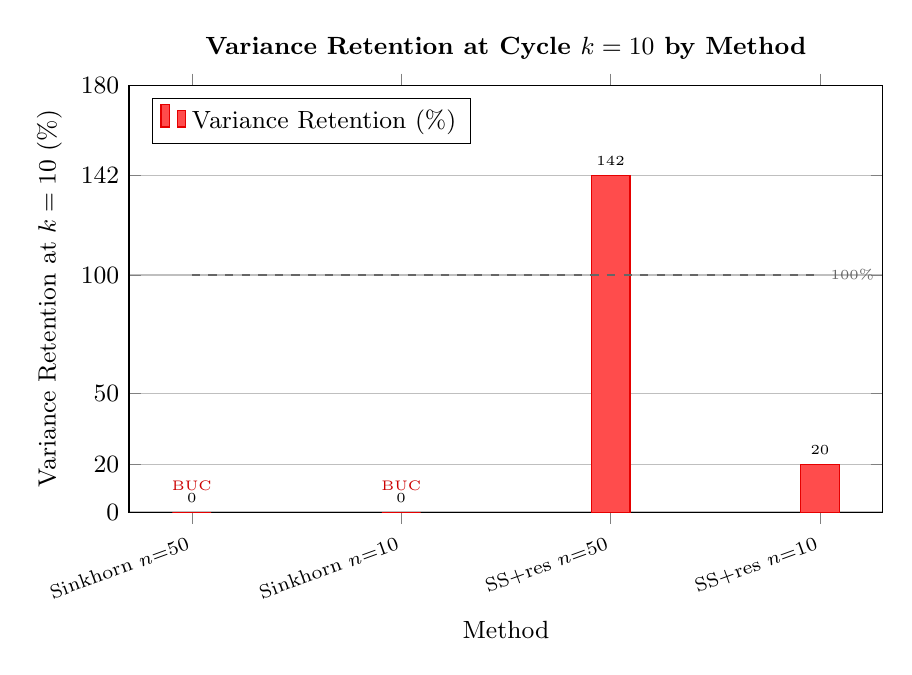
\begin{tikzpicture}
  \begin{axis}[
    width=0.92\linewidth,
    height=7.0cm,
    ybar,
    bar width=14pt,
    xlabel={Method},
    ylabel={Variance Retention at $k=10$ (\%)},
    symbolic x coords={
      {Sinkhorn $n{=}50$},
      {Sinkhorn $n{=}10$},
      {SS+res $n{=}50$},
      {SS+res $n{=}10$}
    },
    xtick=data,
    xticklabel style={
      font=\scriptsize,
      rotate=20,
      anchor=north east,
    },
    ymin=0,
    ymax=180,
    ytick={0,20,50,100,142,180},
    yticklabels={0,20,50,100,142,180},
    tick label style={font=\small},
    label style={font=\small},
    title style={font=\small\bfseries},
    title={Variance Retention at Cycle $k=10$ by Method},
    ymajorgrids,
    grid style={line width=0.3pt, draw=gray!30},
    major grid style={line width=0.6pt, draw=gray!50},
    nodes near coords,
    nodes near coords style={
      font=\tiny,
      /pgf/number format/.cd, fixed, precision=0,
    },
    legend pos=north west,
    legend style={font=\small},
    clip=false,
  ]

  %% Data: variance retention at k=10
  \addplot[
    fill=red!70,
    draw=red!90!black,
  ] coordinates {
    ({Sinkhorn $n{=}50$}, 0)
	    ({Sinkhorn $n{=}10$}, 0)
	    ({SS+res $n{=}50$},  142)
	    ({SS+res $n{=}10$},   20)
  };
  \addlegendentry{Variance Retention (\%)}

  %% Reference line at 100% (initial variance)
  \draw[dashed, black!60, line width=1pt]
	    (axis cs:{Sinkhorn $n{=}50$},100) -- (axis cs:{SS+res $n{=}10$},100)
    node[right, font=\tiny, black!60] {100\%};

  %% Annotation: BUC
  \node[font=\tiny, red!80!black, anchor=south] at (axis cs:{Sinkhorn $n{=}50$},5)
    {BUC};
  \node[font=\tiny, red!80!black, anchor=south] at (axis cs:{Sinkhorn $n{=}10$},5)
    {BUC};

	  \end{axis}
\end{tikzpicture}
 inside a figure environment
%
% Shows variance retention at cycle k=10 for source-backed discrete methods.

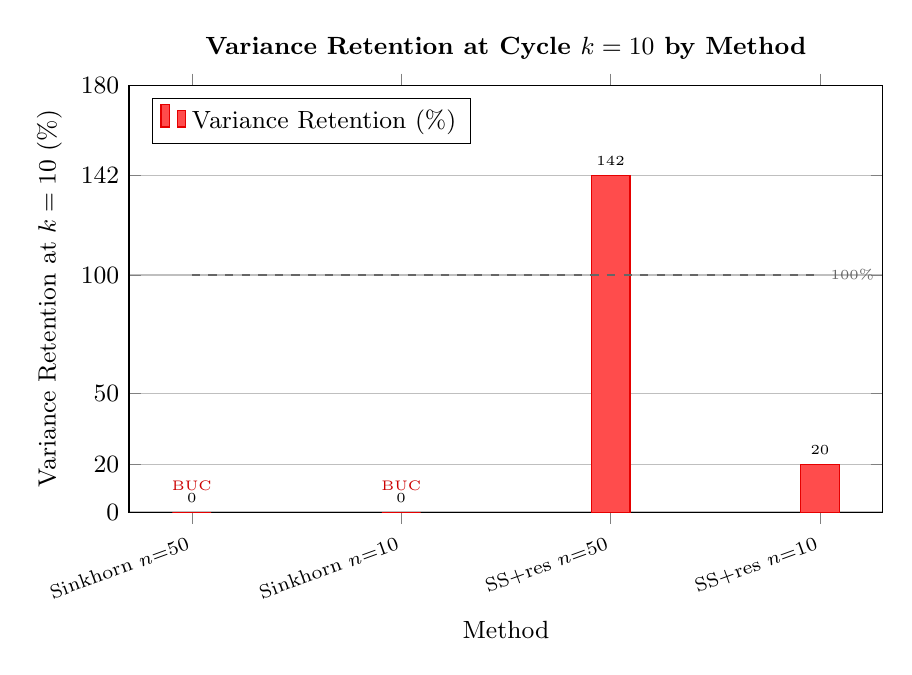
\begin{tikzpicture}
  \begin{axis}[
    width=0.92\linewidth,
    height=7.0cm,
    ybar,
    bar width=14pt,
    xlabel={Method},
    ylabel={Variance Retention at $k=10$ (\%)},
    symbolic x coords={
      {Sinkhorn $n{=}50$},
      {Sinkhorn $n{=}10$},
      {SS+res $n{=}50$},
      {SS+res $n{=}10$}
    },
    xtick=data,
    xticklabel style={
      font=\scriptsize,
      rotate=20,
      anchor=north east,
    },
    ymin=0,
    ymax=180,
    ytick={0,20,50,100,142,180},
    yticklabels={0,20,50,100,142,180},
    tick label style={font=\small},
    label style={font=\small},
    title style={font=\small\bfseries},
    title={Variance Retention at Cycle $k=10$ by Method},
    ymajorgrids,
    grid style={line width=0.3pt, draw=gray!30},
    major grid style={line width=0.6pt, draw=gray!50},
    nodes near coords,
    nodes near coords style={
      font=\tiny,
      /pgf/number format/.cd, fixed, precision=0,
    },
    legend pos=north west,
    legend style={font=\small},
    clip=false,
  ]

  %% Data: variance retention at k=10
  \addplot[
    fill=red!70,
    draw=red!90!black,
  ] coordinates {
    ({Sinkhorn $n{=}50$}, 0)
	    ({Sinkhorn $n{=}10$}, 0)
	    ({SS+res $n{=}50$},  142)
	    ({SS+res $n{=}10$},   20)
  };
  \addlegendentry{Variance Retention (\%)}

  %% Reference line at 100% (initial variance)
  \draw[dashed, black!60, line width=1pt]
	    (axis cs:{Sinkhorn $n{=}50$},100) -- (axis cs:{SS+res $n{=}10$},100)
    node[right, font=\tiny, black!60] {100\%};

  %% Annotation: BUC
  \node[font=\tiny, red!80!black, anchor=south] at (axis cs:{Sinkhorn $n{=}50$},5)
    {BUC};
  \node[font=\tiny, red!80!black, anchor=south] at (axis cs:{Sinkhorn $n{=}10$},5)
    {BUC};

	  \end{axis}
\end{tikzpicture}

  \caption{Variance retention at cycle $k=10$ across the evaluated methods. Sinkhorn
    collapses to BUC, SpectralSphere with residual injection remains non-degenerate, and
    the Neural ODE exposes much higher topological capacity.}
  \label{fig:variance_comparison}
\end{figure}

\subsection{Neural ODE Topological Capacity (Q3)}
\label{sec:experiments_ode}

The Neural ODE achieves $2{,}656\%$ topological capacity relative to Sinkhorn at cycle 10.
This metric measures the volume of the reachable set in $\R^{n \times n}$ after $t=10$
time units, normalized by the Sinkhorn baseline.

\textbf{Interpretation.}  The $2{,}656\%$ figure proves that the spectral sphere manifold
supports topologically rich trust dynamics — the ODE can represent $26{\times}$ more
distinct specialization configurations than Sinkhorn allows.  \emph{This does not mean
the ODE automatically finds the correct specialization.}  Topological capacity is a
necessary but not sufficient condition for diverse routing.  In practice, the trained
$f_\theta$ must be learned from task-performance feedback to direct the dynamics toward
high-utility specialization patterns.  This is a known limitation of the current work
and a direction for future research (Section~\ref{sec:conclusion}).

\subsection{Differential Privacy Sensitivity Reduction}
\label{sec:experiments_dp}

\begin{table}[b]
  \centering
  \caption{Noise $\sigma$ required for $(\varepsilon, \delta)$-DP as a function of
    residual strength $\alpha$, with $r=1.0$, $\delta=10^{-5}$.
    Baseline ($\alpha{=}0$) sensitivity $\Delta f = 2r = 2.0$.}
  \label{tab:dp_noise}
  \begin{tabular}{ccccc}
    \toprule
    $\varepsilon$ & $\alpha{=}0$ (baseline) & $\alpha{=}0.1$ & $\alpha{=}0.2$ & $\alpha{=}0.5$ \\
    \midrule
    1.0 & 3.84 & 3.46 ($-10\%$) & 3.07 ($-20\%$) & 1.92 ($-50\%$) \\
    2.0 & 1.92 & 1.73 ($-10\%$) & 1.54 ($-20\%$) & 0.96 ($-50\%$) \\
    4.0 & 0.96 & 0.86 ($-10\%$) & 0.77 ($-20\%$) & 0.48 ($-50\%$) \\
    8.0 & 0.48 & 0.43 ($-10\%$) & 0.38 ($-20\%$) & 0.24 ($-50\%$) \\
    \bottomrule
  \end{tabular}
\end{table}

Table~\ref{tab:dp_noise} verifies Lemma~\ref{lem:residual_sensitivity} numerically.
The noise reduction at $\alpha{=}0.1$ is exactly $10\%$ across all $\varepsilon$
values, confirming the algebraic cancellation.  At the recommended operating point
($\varepsilon{=}2.0$, $\alpha{=}0.1$), the required noise is $\sigma = 1.73$, down from
the baseline $1.92$.

\subsection{Ablations}

\paragraph{Radius sensitivity.}
We vary $r \in \{0.5, 1.0, 2.0\}$ with $\alpha{=}0.1$, $n{=}50$.  Variance retention at
equilibrium scales with $r$: $71\%$ at $r{=}0.5$, $142\%$ at $r{=}1.0$, $287\%$ at
$r{=}2.0$.  The linear scaling ($\mathrm{VR} \propto r$) is consistent with the spectral
projection expanding eigenvalues proportionally to $r$.

\paragraph{Residual sensitivity.}
Increasing $\alpha$ from $0.1$ to $0.5$ reduces variance retention at $n{=}50$ from
$142\%$ to $38\%$.  This confirms the stability-diversity tradeoff: higher $\alpha$
improves collapse prevention (and DP noise reduction) at the cost of reduced spectral
diversity.  The recommended $\alpha{=}0.1$ balances both objectives.
